\documentclass{beamer}

\usepackage{graphicx}
\usepackage{fontspec}
\usepackage[scale=0.9,sfdefault,light]{roboto}
\usepackage{listings}

\definecolor{unusedline}{gray}{0.7}

\graphicspath{ {img/} }

\usetheme{Marburg}
\usecolortheme{whale}

\title{git essential}
\subtitle{git essential}
\date{\today}

\begin{document}

\begin{frame}
    \begin{figure}
        \center
        
\includegraphics{git-logo}
        \label{fig:git-logo}
    \end{figure}
    \center{git essential}
    \center{ \tiny{Sitdhibong Laokok} }
\end{frame}

\begin{frame}
    \begin{figure}
        \center
        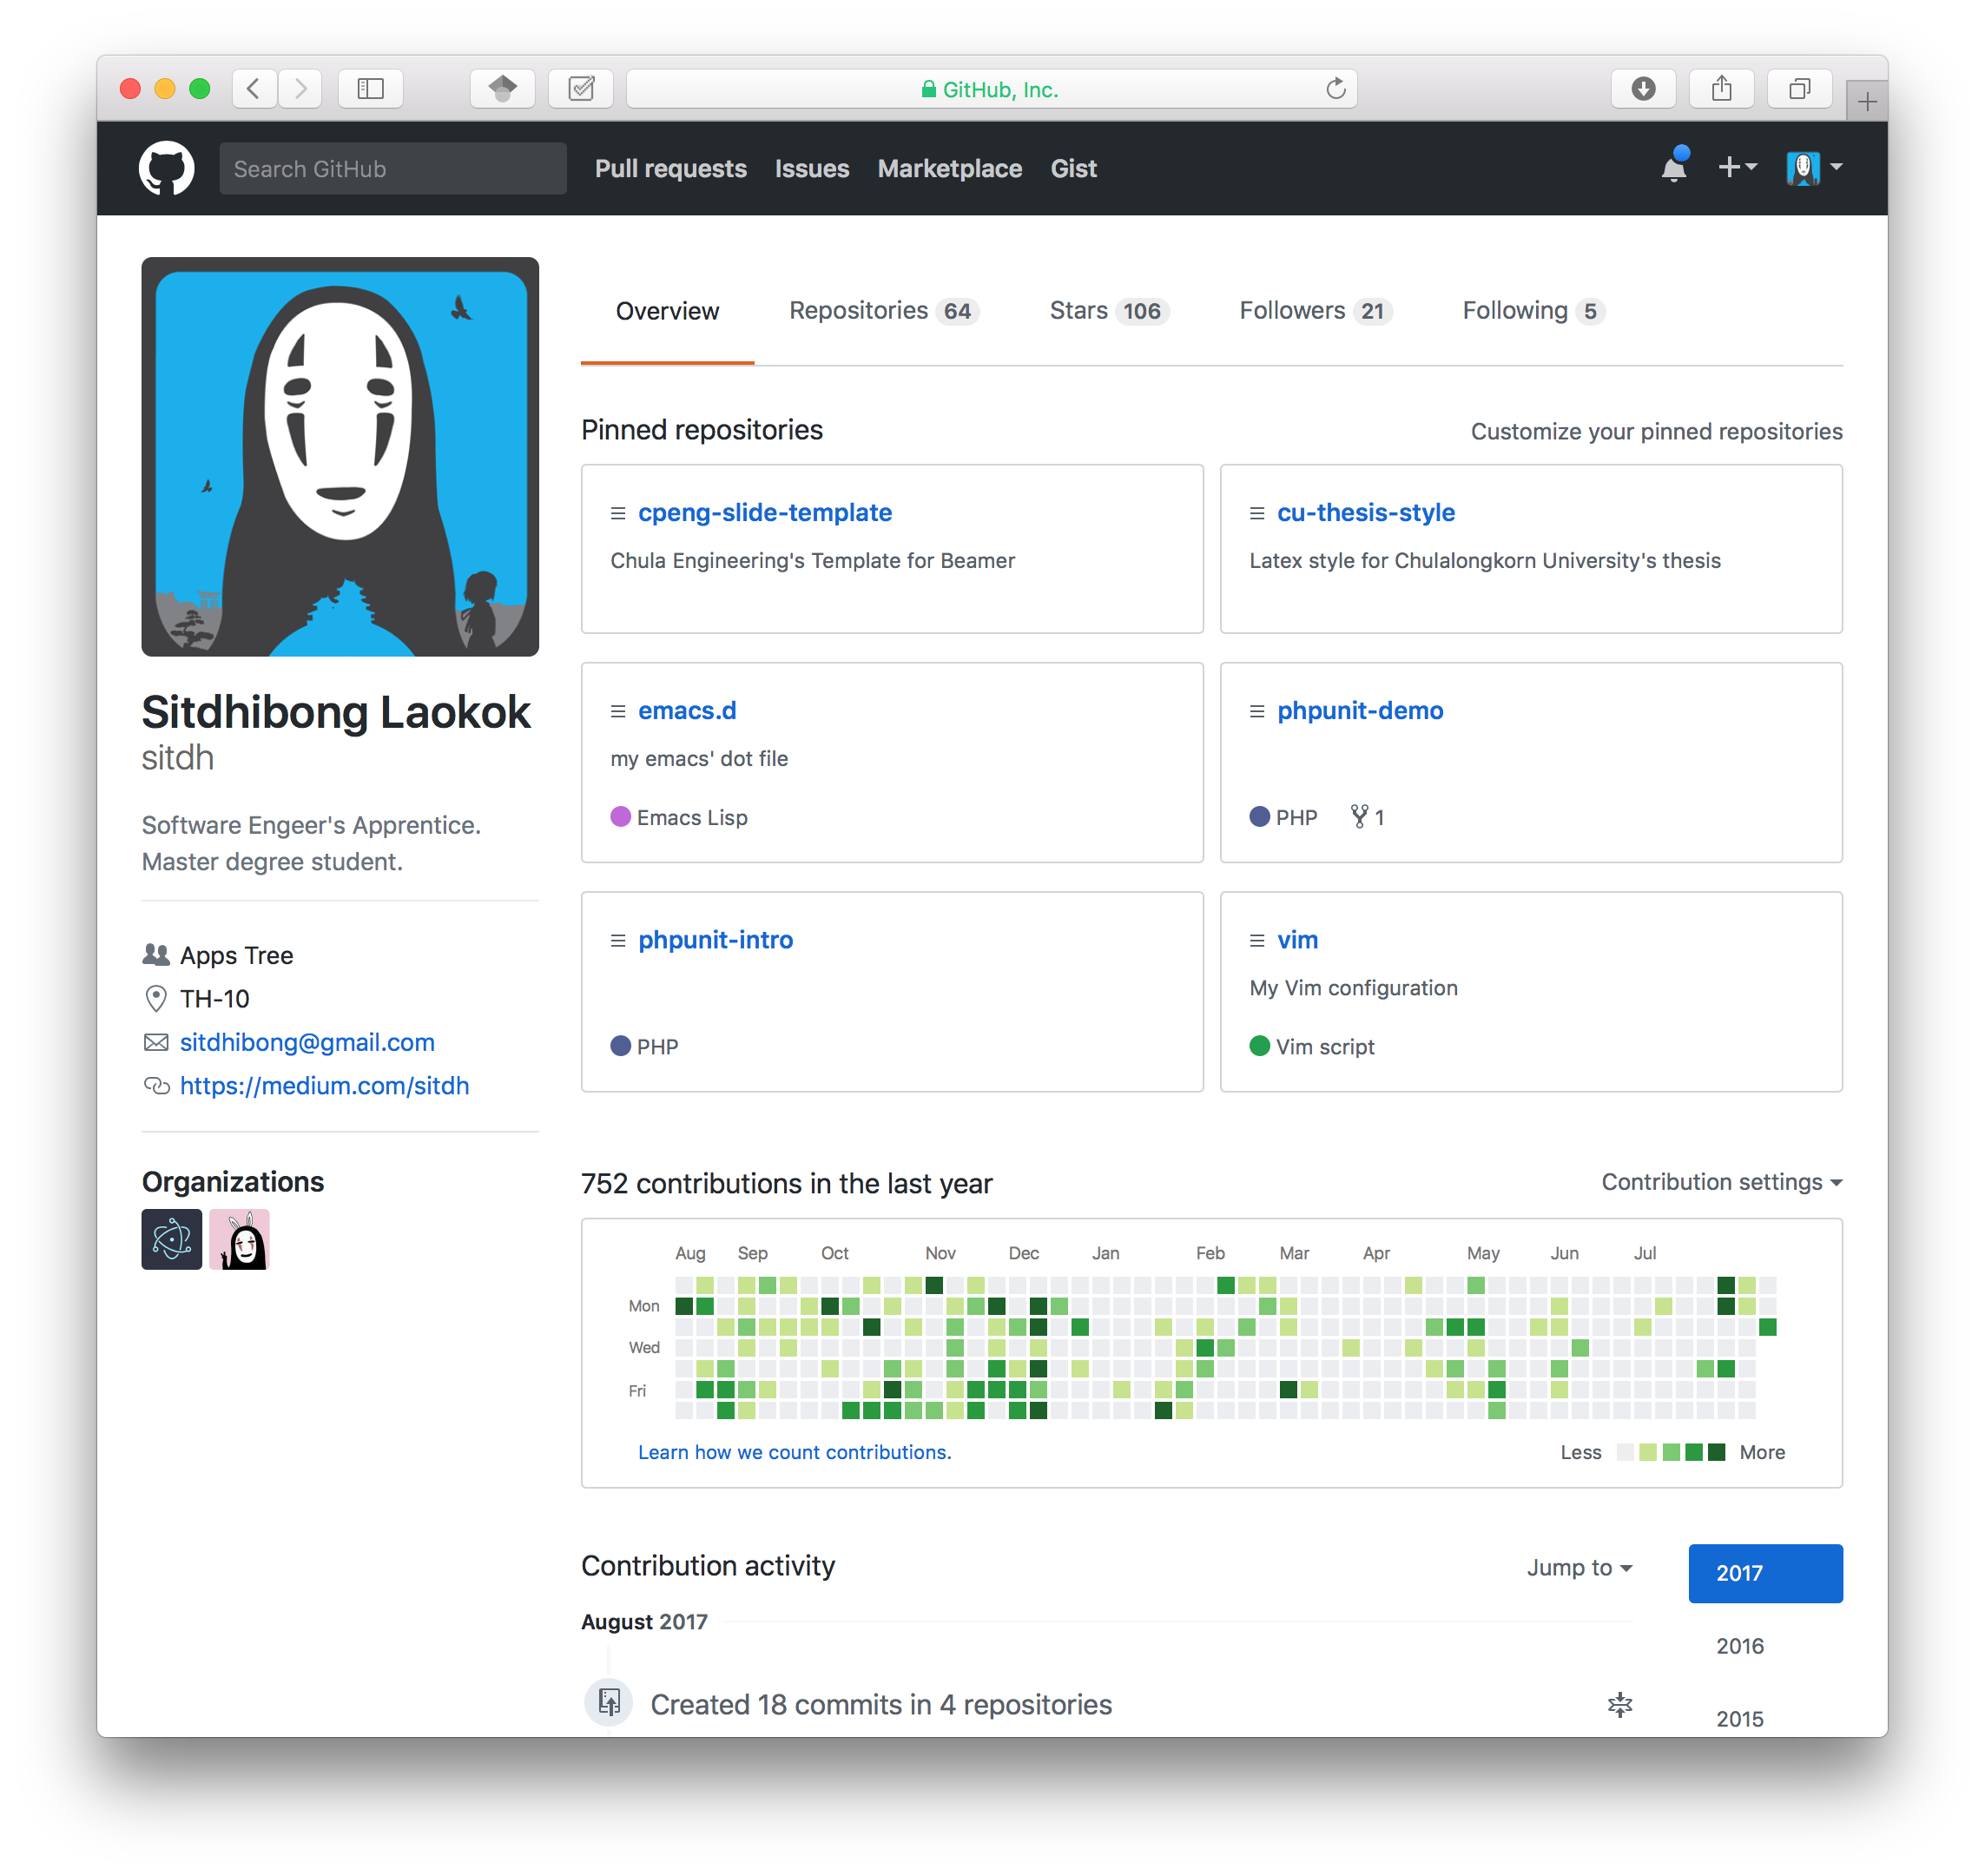
\includegraphics[width=.8\textwidth]{git-profile}
        \caption{https://github.com/sitdh}
        \label{fig:git-profile}
    \end{figure}
\end{frame}

\begin{frame}
    \frametitle{Outline}
    \tableofcontents
\end{frame}

\section{Activity flow}
\begin{frame}{Activity flow}
    \begin{figure}
        \center
        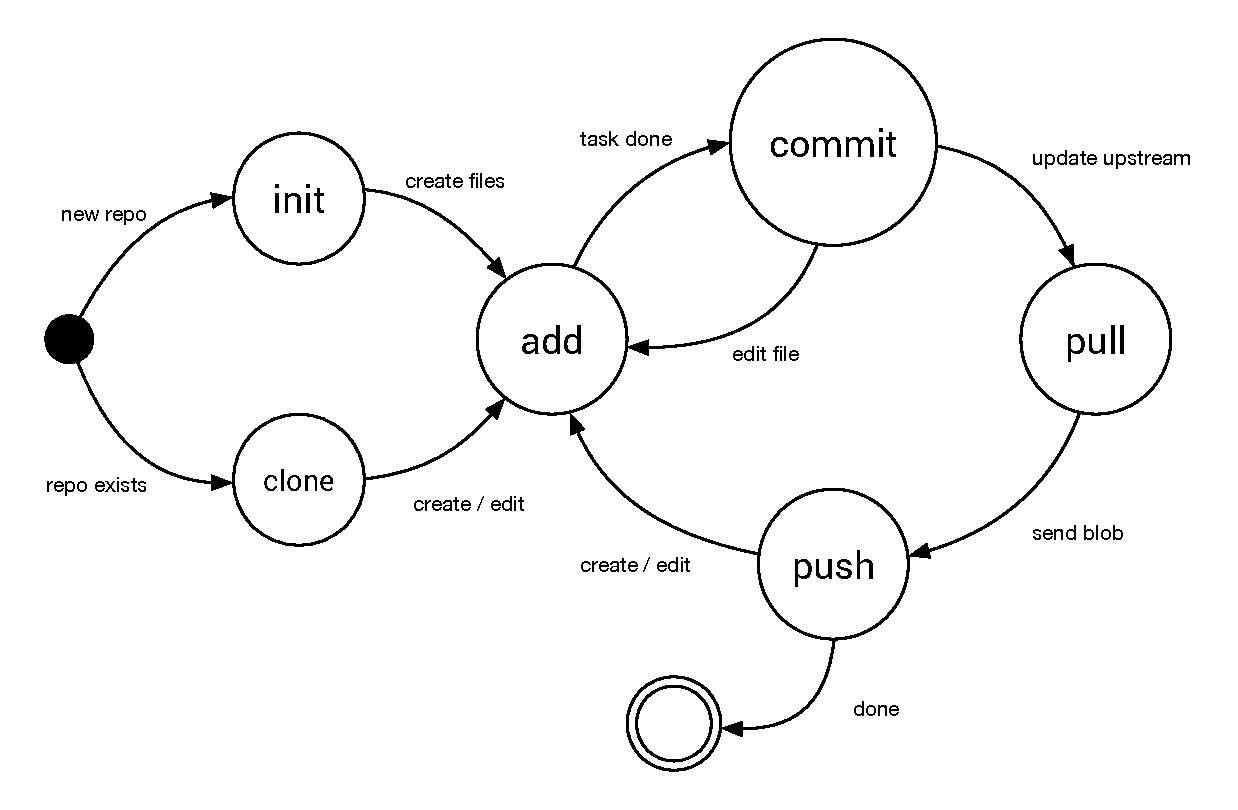
\includegraphics[width=.9\textwidth]{git-command-flow}
        \label{fig:git-command-flow}
    \end{figure}
\end{frame}

\subsection{init}
\begin{frame}{init}
    \Large{\$ git init}
    \begin{figure}
        \center
        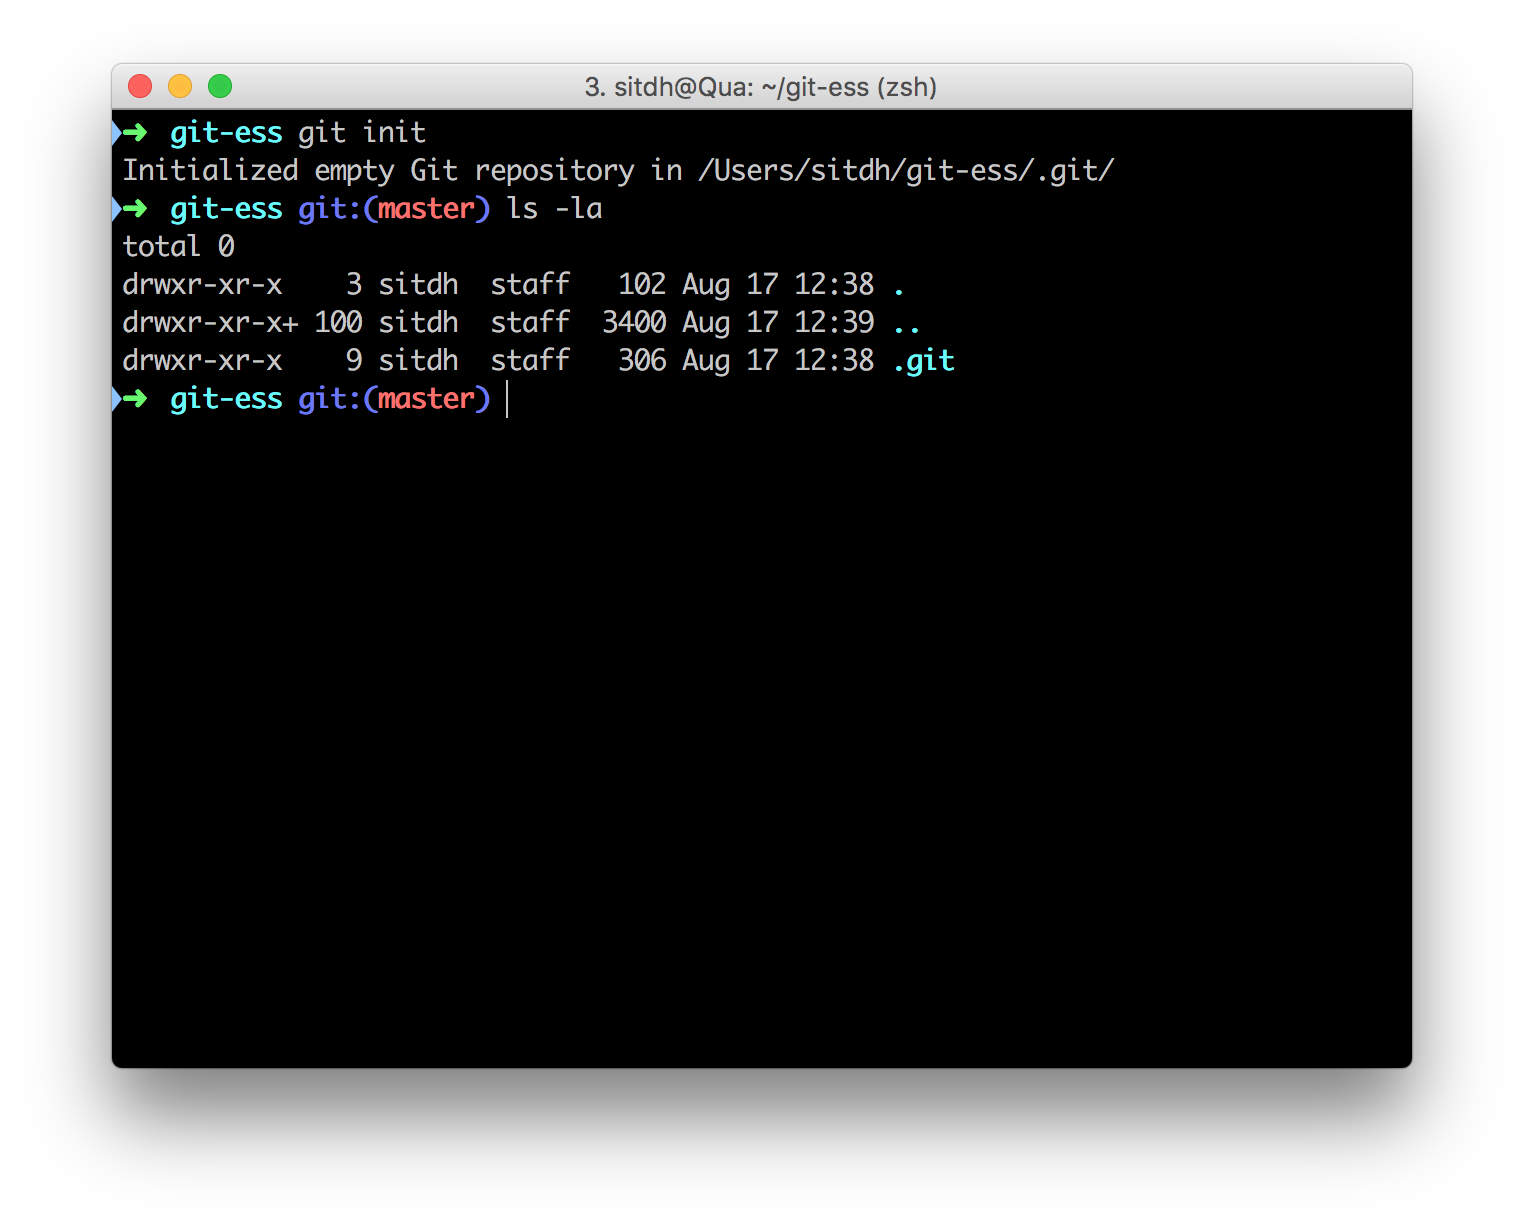
\includegraphics[width=.9\textwidth]{git-init}
        \label{fig:git-init}
    \end{figure}
\end{frame}

\begin{frame}{init -\,-bare}
    \Large{\$ git init -\,-bare}
    \begin{figure}
        \center
        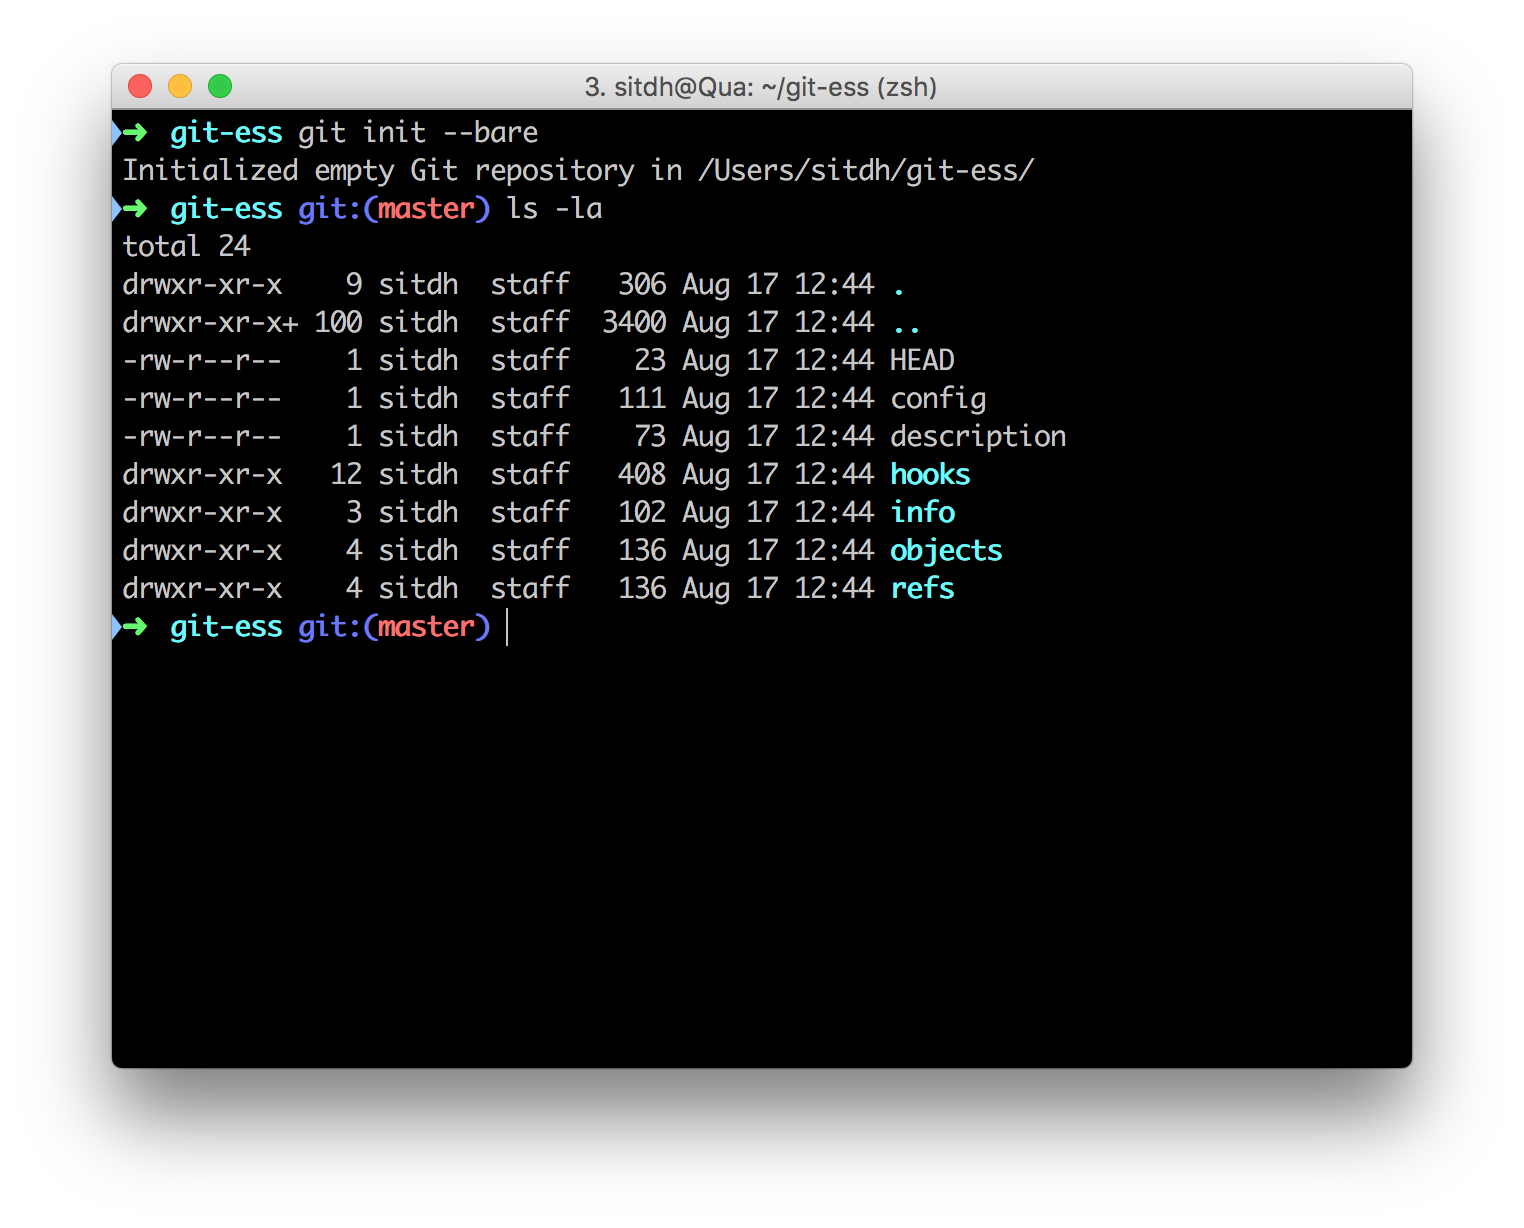
\includegraphics[width=.9\textwidth]{git-init--bare}
        \label{fig:git-init--bare}
    \end{figure}
\end{frame}

\subsection[clone]{clone}
\begin{frame}{clone}
    \begin{figure}
        \center
        \includegraphics<1>[width=.7\textwidth]{git-clone-action-0}
        \includegraphics<2>[width=.7\textwidth]{git-clone-action-1}
    \end{figure}
\end{frame}

\begin{frame}{clone}
    \only<1->{
        \textcolor<2->{gray}{\,\,\,\,\Large{\$ git clone \em{"Repo" ["Dest"]}} \newline}
    }
    \only<2->{
        \Large{\$ git clone \textcolor<3>{red}{\,git-ess} \textcolor<4>{red}{\,gitess}}
    }
    \begin{figure}
        \center
        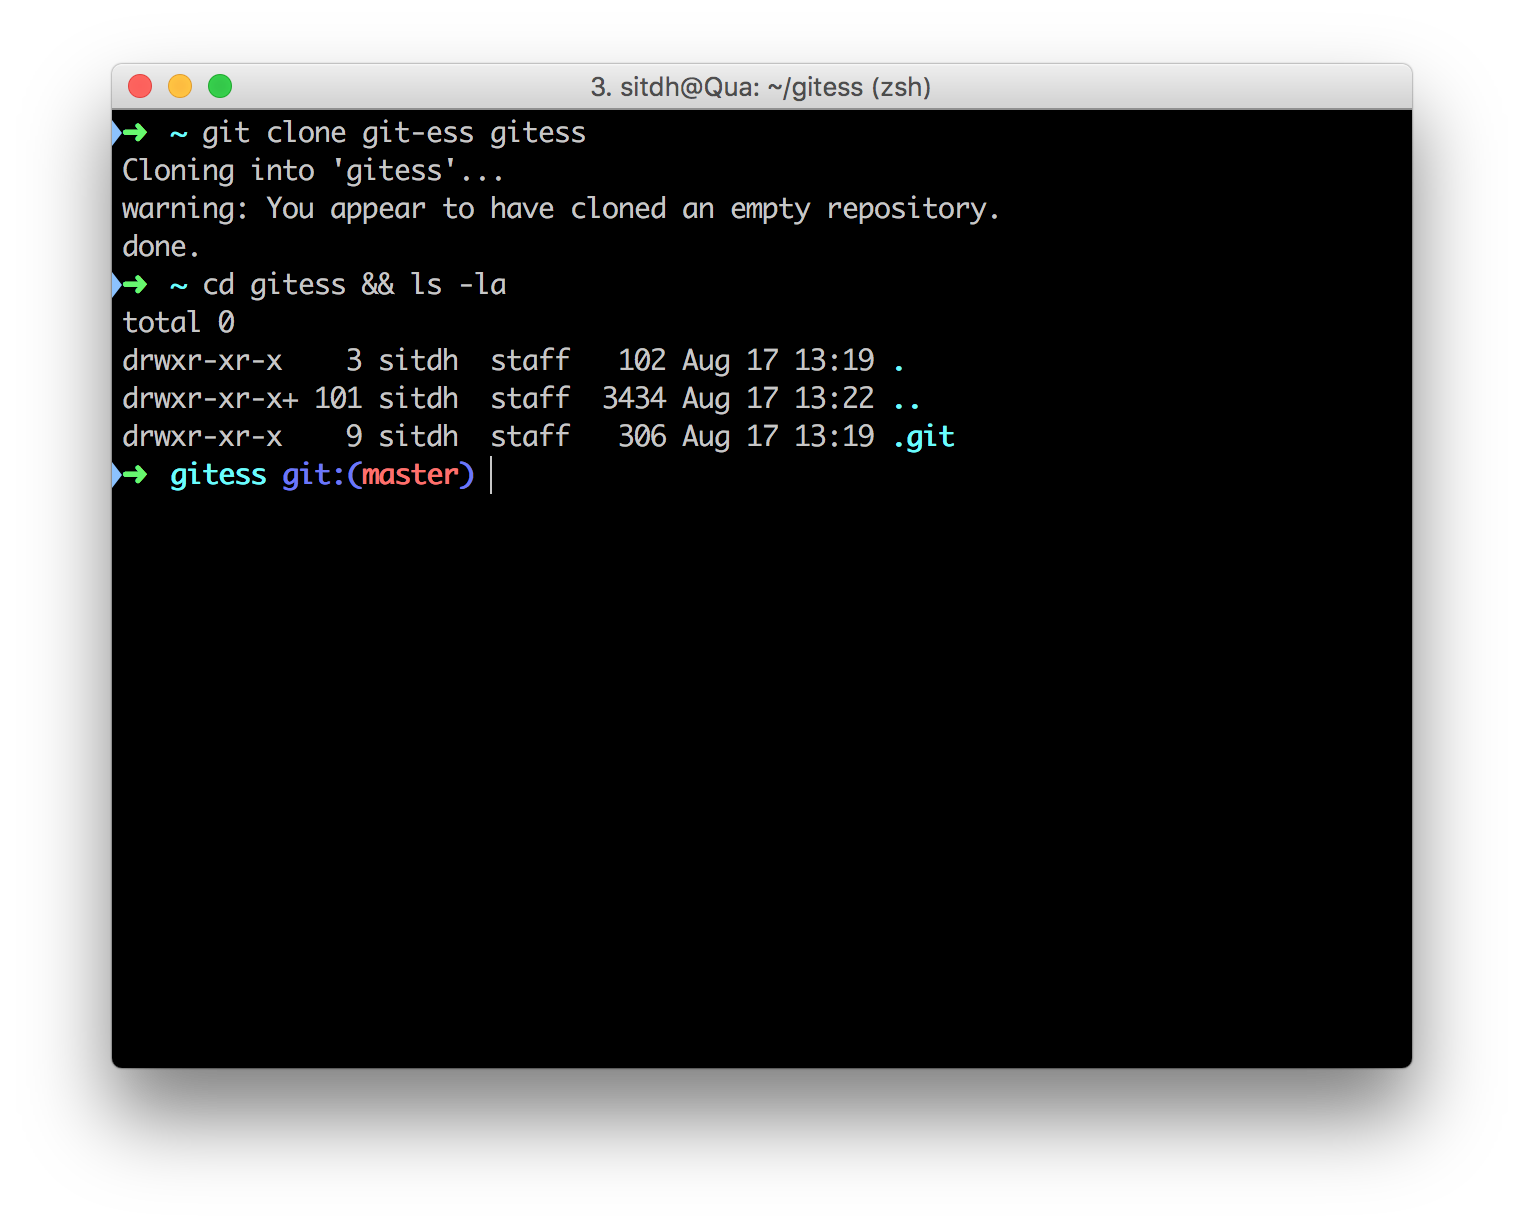
\includegraphics[width=.9\textwidth]{git-clone}
        \label{fig:git-clone}
    \end{figure}
\end{frame}

\subsection[add]{add}
\begin{frame}{Activity flow}
    \begin{figure}
        \center
        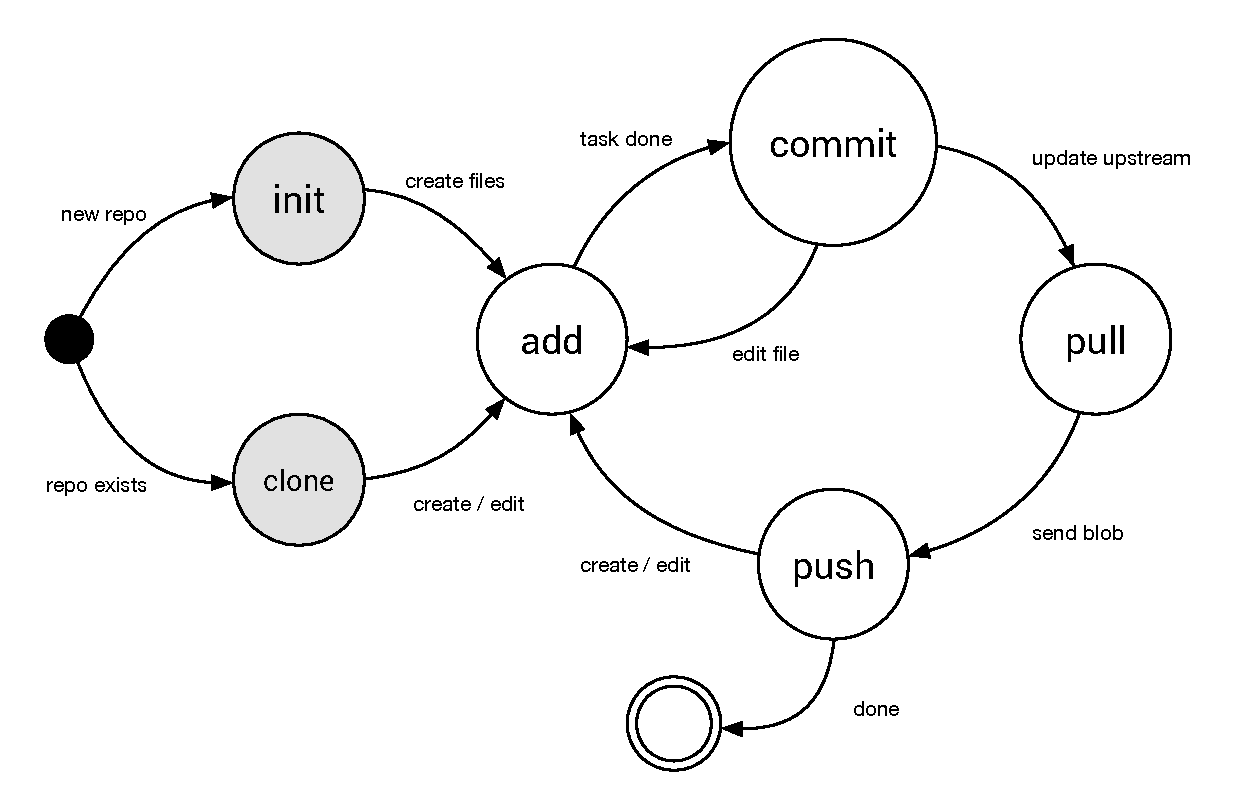
\includegraphics[width=.9\textwidth]{git-command-flow-1}
        \label{fig:git-command-flow-1}
    \end{figure}
\end{frame}

\begin{frame}{unstage \& staged}
    \begin{figure}
        \center
        \includegraphics<1>[width=.8\textwidth]{project-changed-0}
        \includegraphics<2>[width=.8\textwidth]{project-changed-1}
        \includegraphics<3>[width=.8\textwidth]{project-changed-2}
        \includegraphics<4>[width=.8\textwidth]{project-changed-3-2}
        \includegraphics<5>[width=.8\textwidth]{project-changed-3-1}
        \includegraphics<6>[width=.8\textwidth]{project-changed-4}
        \label{fig:project-changed}
    \end{figure}
    \small{https://git-scm.com/book/en/v2/Git-Basics-Recording-Changes-to-the-Repository}
\end{frame}

\begin{frame}{add}
    \only<1->{\textcolor<2>{gray}{\Large{\$ git add \em{/opt/path}} \newline\newline}}
    \only<2>{\Large{\$ git add .}}
\end{frame}

\subsection[commit]{commit}
\begin{frame}{Activity flow}
    \begin{figure}
        \center
        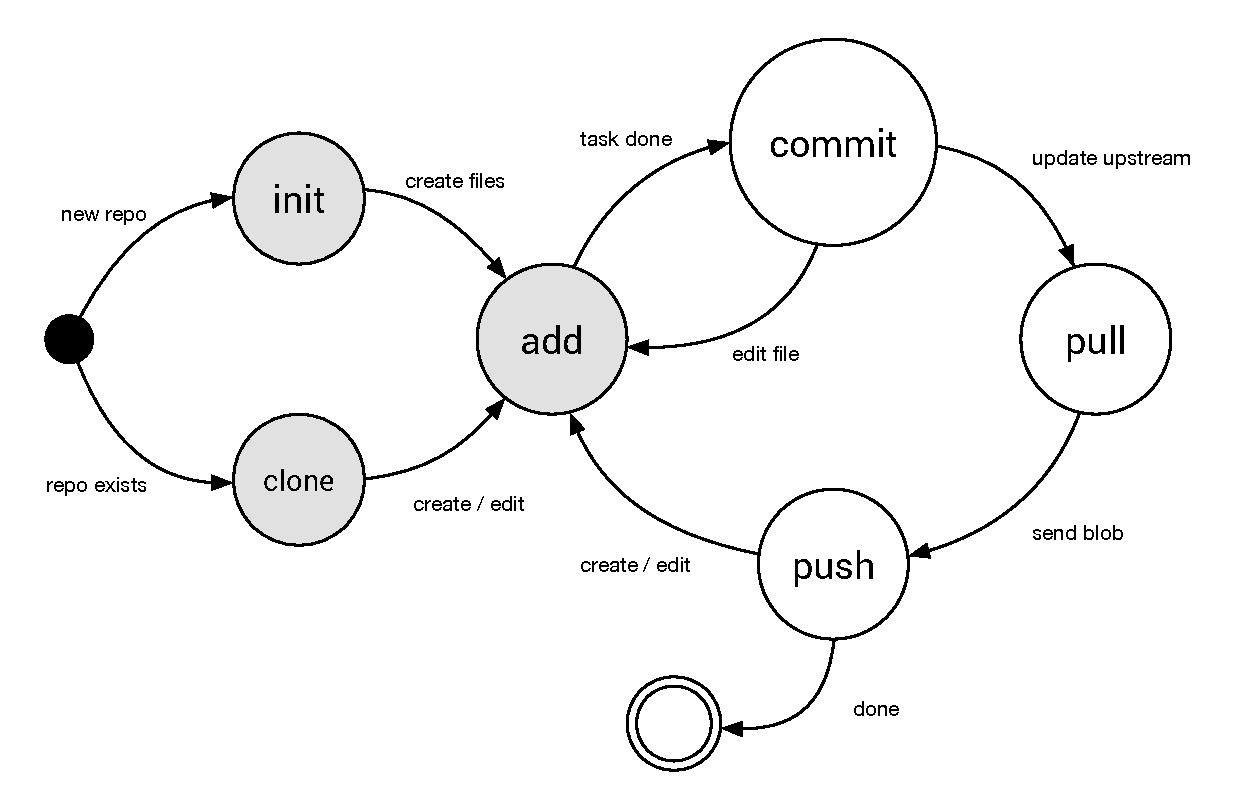
\includegraphics[width=.9\textwidth]{git-command-flow-2}
        \label{fig:git-command-flow-2}
    \end{figure}
\end{frame}

\begin{frame}{commit}
    \begin{figure}
        \center
        \includegraphics<1>[width=.8\textwidth]{project-changed-0}
        \includegraphics<2>[width=.8\textwidth]{project-changed-1}
        \includegraphics<3>[width=.8\textwidth]{project-changed-2}
        \label{fig:project-changed-2}
    \end{figure}
\end{frame}

\begin{frame}{commit}
    \begin{figure}
        \center
        \includegraphics<1>[width=.8\textwidth]{git-commit-flow-1}
        \includegraphics<2>[width=.8\textwidth]{git-commit-flow-2-1}
        \includegraphics<3>[width=.8\textwidth]{git-commit-flow-2-2}
        \includegraphics<4>[width=.8\textwidth]{git-commit-flow-3}
        \includegraphics<5>[width=.8\textwidth]{git-commit-flow-4}
        \includegraphics<6>[width=.8\textwidth]{git-commit-flow-4-1}
        \label{fig:git-commit-flow}
    \end{figure}
\end{frame}

\begin{frame}{commit}
    \only<1->{
        \Large{\textcolor<3->{gray}{\$ git commit -am \textcolor<2>{blue}{"Commit message"}}} \newline
    }
    \only<3->{
        \Large{\$ git commit -m \textcolor<4->{blue}{"Update lib version for issue \#32"} \textcolor<5->{red}{config.json}
        }
    }
\end{frame}

\begin{frame}[t]{commit message}
    \begin{enumerate}
        \item<1-> \textcolor<3->{gray}{Separate subject from body with a blank line}
        \item<3-> \textcolor<6->{gray}{Limit the subject line to 50 characters \newline 
            and wrap the body at 72 characters}
        \item<6-> \textcolor<9->{gray}{Capitalize the subject line}
        \item<9-> \textcolor<10->{gray}{Do not end the subject line with a period}
        \item<10-> \textcolor<13->{gray}{Use the imperative mood in the subject line}
        \item<13-> Use the body to explain \texttt{what} and \texttt{why} vs. \texttt{how}
    \end{enumerate}

    % Heading 
    \only<2>{
        \textbf{Derezz the master control program} \newline

        MCP turned out to be evil and had become intent on world domination.
        This commit throws Tron's disc into MCP (causing its deresolution)
        and turns it back into a chess game.
    }

    % Limit
    \only<4>{
        {\par
        MCP turned out to be evil and had become intent on world domination. This commit throws Tron's disc into MCP (causing its deresolution) and turns it back into a chess game.}
    }

    \only<5>{Derezz the master control program}

    % Capitalize
    \only<7-8>{\textcolor<8>{red}{fix issue \#27} \newline}
    \only<8>{Fix issue \#27}

    % Imperative mood
    \only<11>{\em "Spoken or written as if giving a command or instruction"}
    \only<12>{ 
        \begin{itemize}
            \item Close the door
            \item Take out the trash
            \item Merge branch 'feature'
        \end{itemize}
    }

    % What, Why and How
    \only<14>{
        \begin{itemize}
            \item What side effects does this change have? 
            \item Why is this change necessary?
            \item How does it address the issue?
        \end{itemize}
    }
\end{frame}

\subsection[pull]{pull}
\begin{frame}{Activity flow}
    \begin{figure}
        \center
        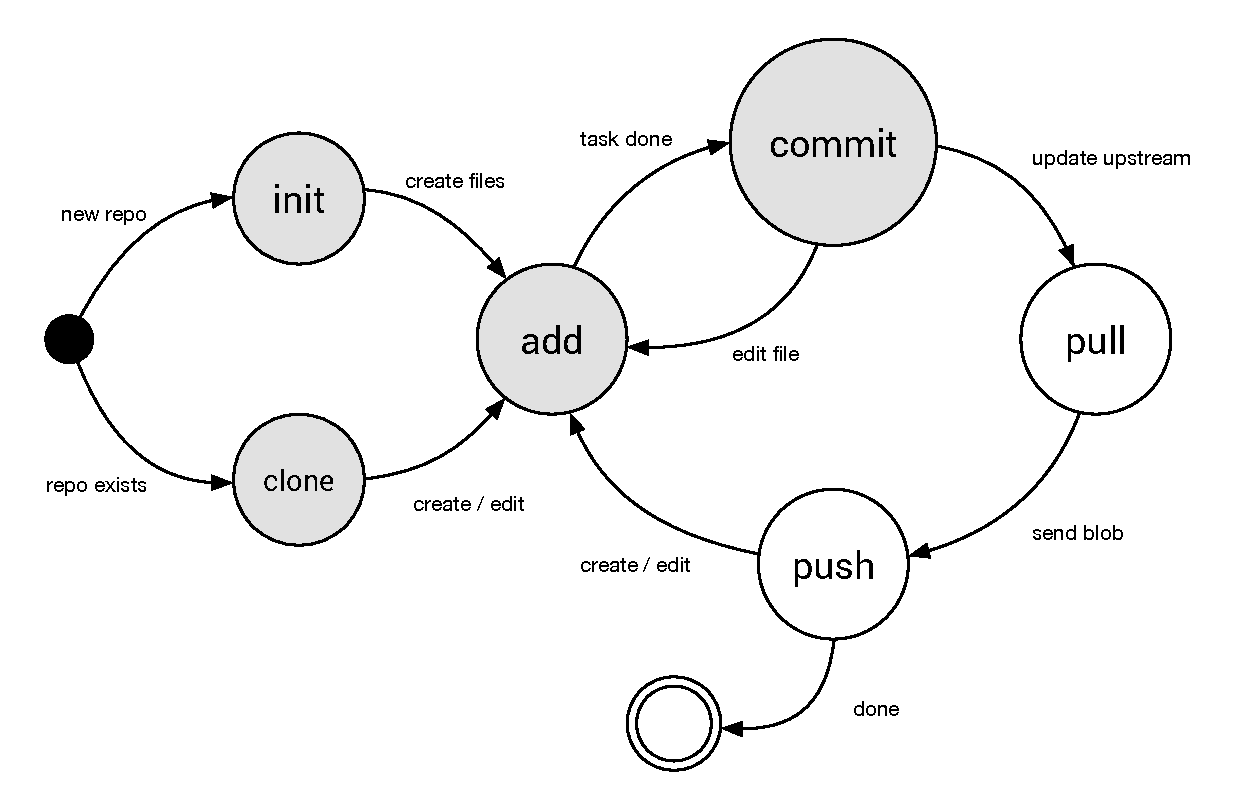
\includegraphics[width=.9\textwidth]{git-command-flow-3}
        \label{fig:git-command-flow-3}
    \end{figure}
\end{frame}

\begin{frame}{pull - Sync information}
    \begin{figure}
        \center
        \includegraphics<1>[width=.7\textwidth]{git-pulling-information-0}
        \includegraphics<2>[width=.7\textwidth]{git-pulling-information-1}
        \label{fig:git-pulling-information}
    \end{figure}
\end{frame}

\begin{frame}{pull}
    \only{
        \Large{
            \[
                Pull = Fetch + Merge
            \]
        }
    }
\end{frame}

\subsection{push}
\begin{frame}{Activity flow}
    \begin{figure}
        \center
        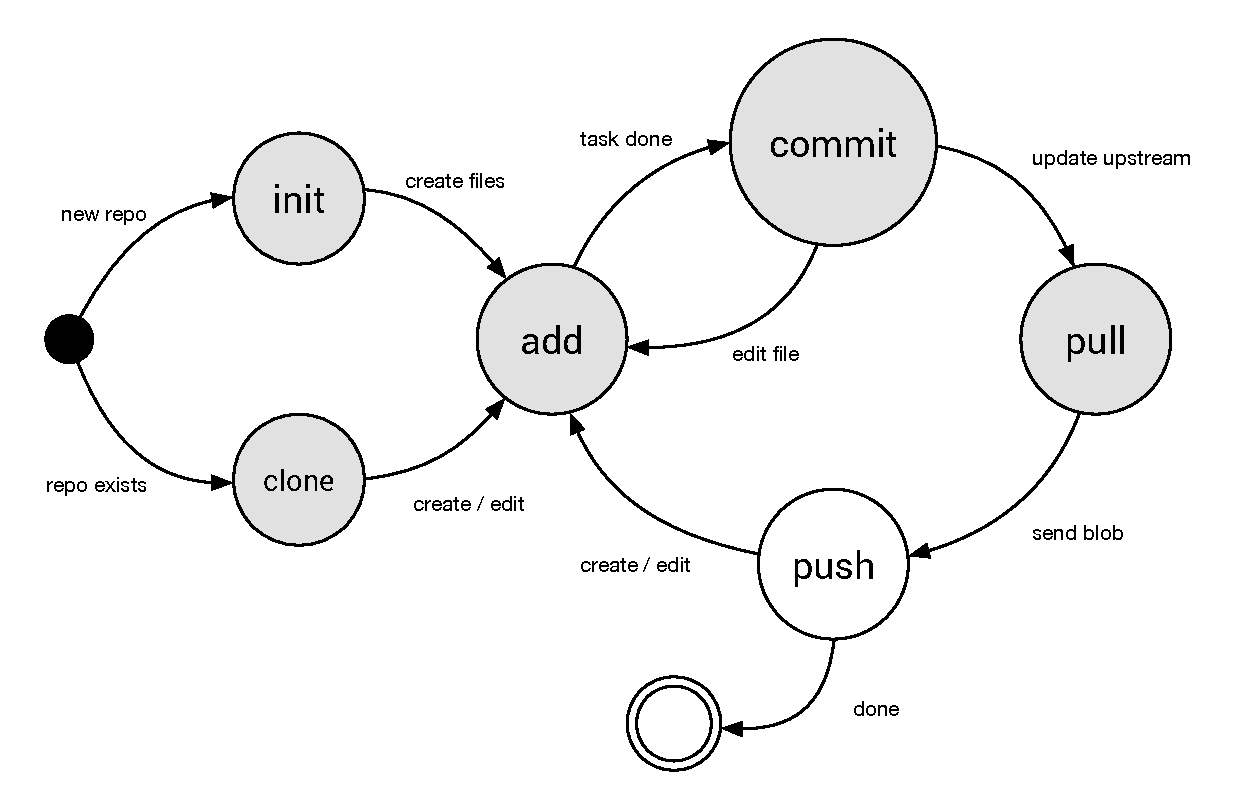
\includegraphics[width=.9\textwidth]{git-command-flow-4}
        \label{fig:git-command-flow-4}
    \end{figure}
\end{frame}

\section[branch]{branch}
\begin{frame}{Recommand branches}
    \begin{figure}
        \center
        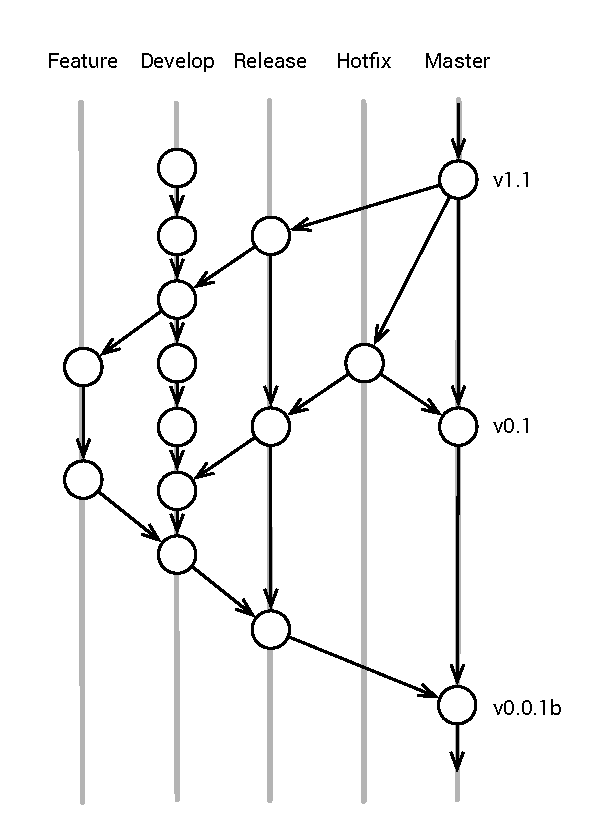
\includegraphics[height=.8\textheight]{git-recommanded-branches}
        \label{fig:git-recommanded-branches}
    \end{figure}
\end{frame}

\begin{frame}{git-flow}
    \begin{figure}
        \center
        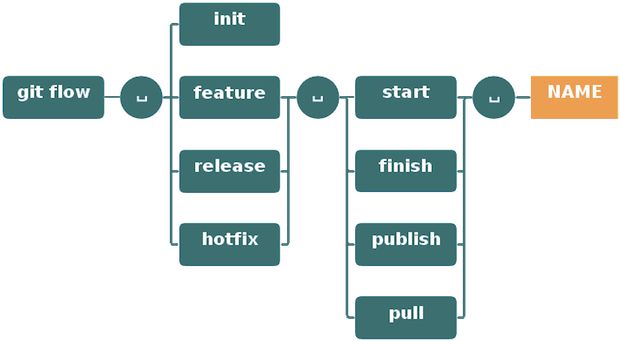
\includegraphics[width=.9\textwidth]{git-flow-commands}
        \label{fig:git-flow-commands}
    \end{figure}
    \center{https://danielkummer.github.io/git-flow-cheatsheet/}
\end{frame}

\begin{frame}{push}
\end{frame}

\section{Checkup}
\begin{frame}
    \frametitle{Checkup}
    \begin{figure}
        \center
        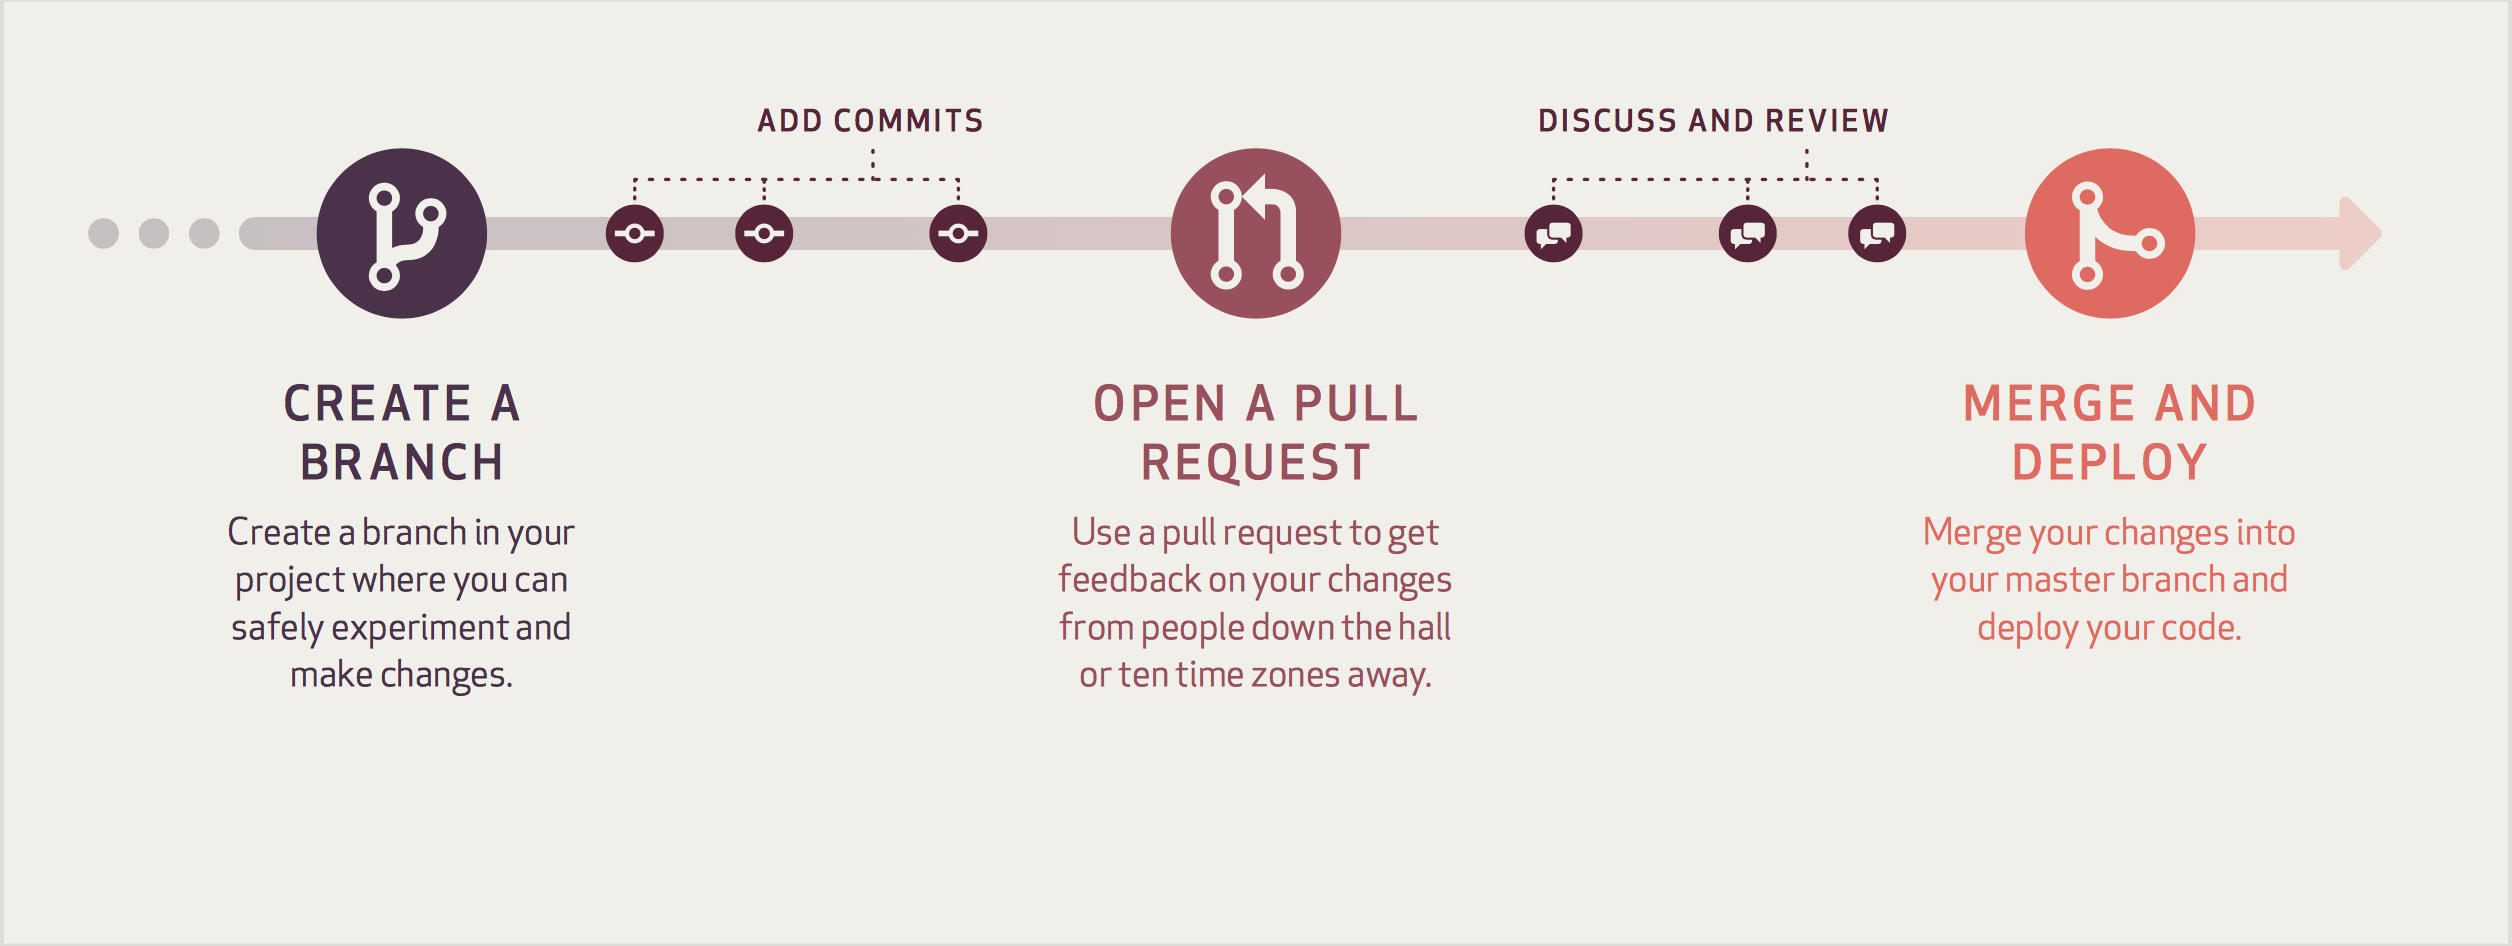
\includegraphics[width=.9\textwidth]{git-workflow}
        \caption{https://guides.github.com/introduction/flow/}
        \label{fig:git-workflow}
    \end{figure}
\end{frame}

\section[workshop]{Workshop}
\begin{frame}{GitHub - Happy coding}
    \begin{itemize}
        \item Create local repository
        \item Add and commit files
        \item Create Remote repository on GitHub
        \item Collaboration overview
    \end{itemize}
\end{frame}

\begin{frame}{Create local repository}
\end{frame}

\begin{frame}{Add and commit files}
\end{frame}

\begin{frame}{Create remote repository on GitHub}
\end{frame}

\begin{frame}{Collaboration overview}
\end{frame}

\end{document}
